\chapter{Design and construction of experimental apparatus}
\label{beamline}

\section{Introduction}
\label{intro_beamline}


\section{Beamline}
\label{sec:full_beamline}

\subsection{Time Delay Control}
\label{sec:delay_wedges}

\begin{figure}
	\centering
	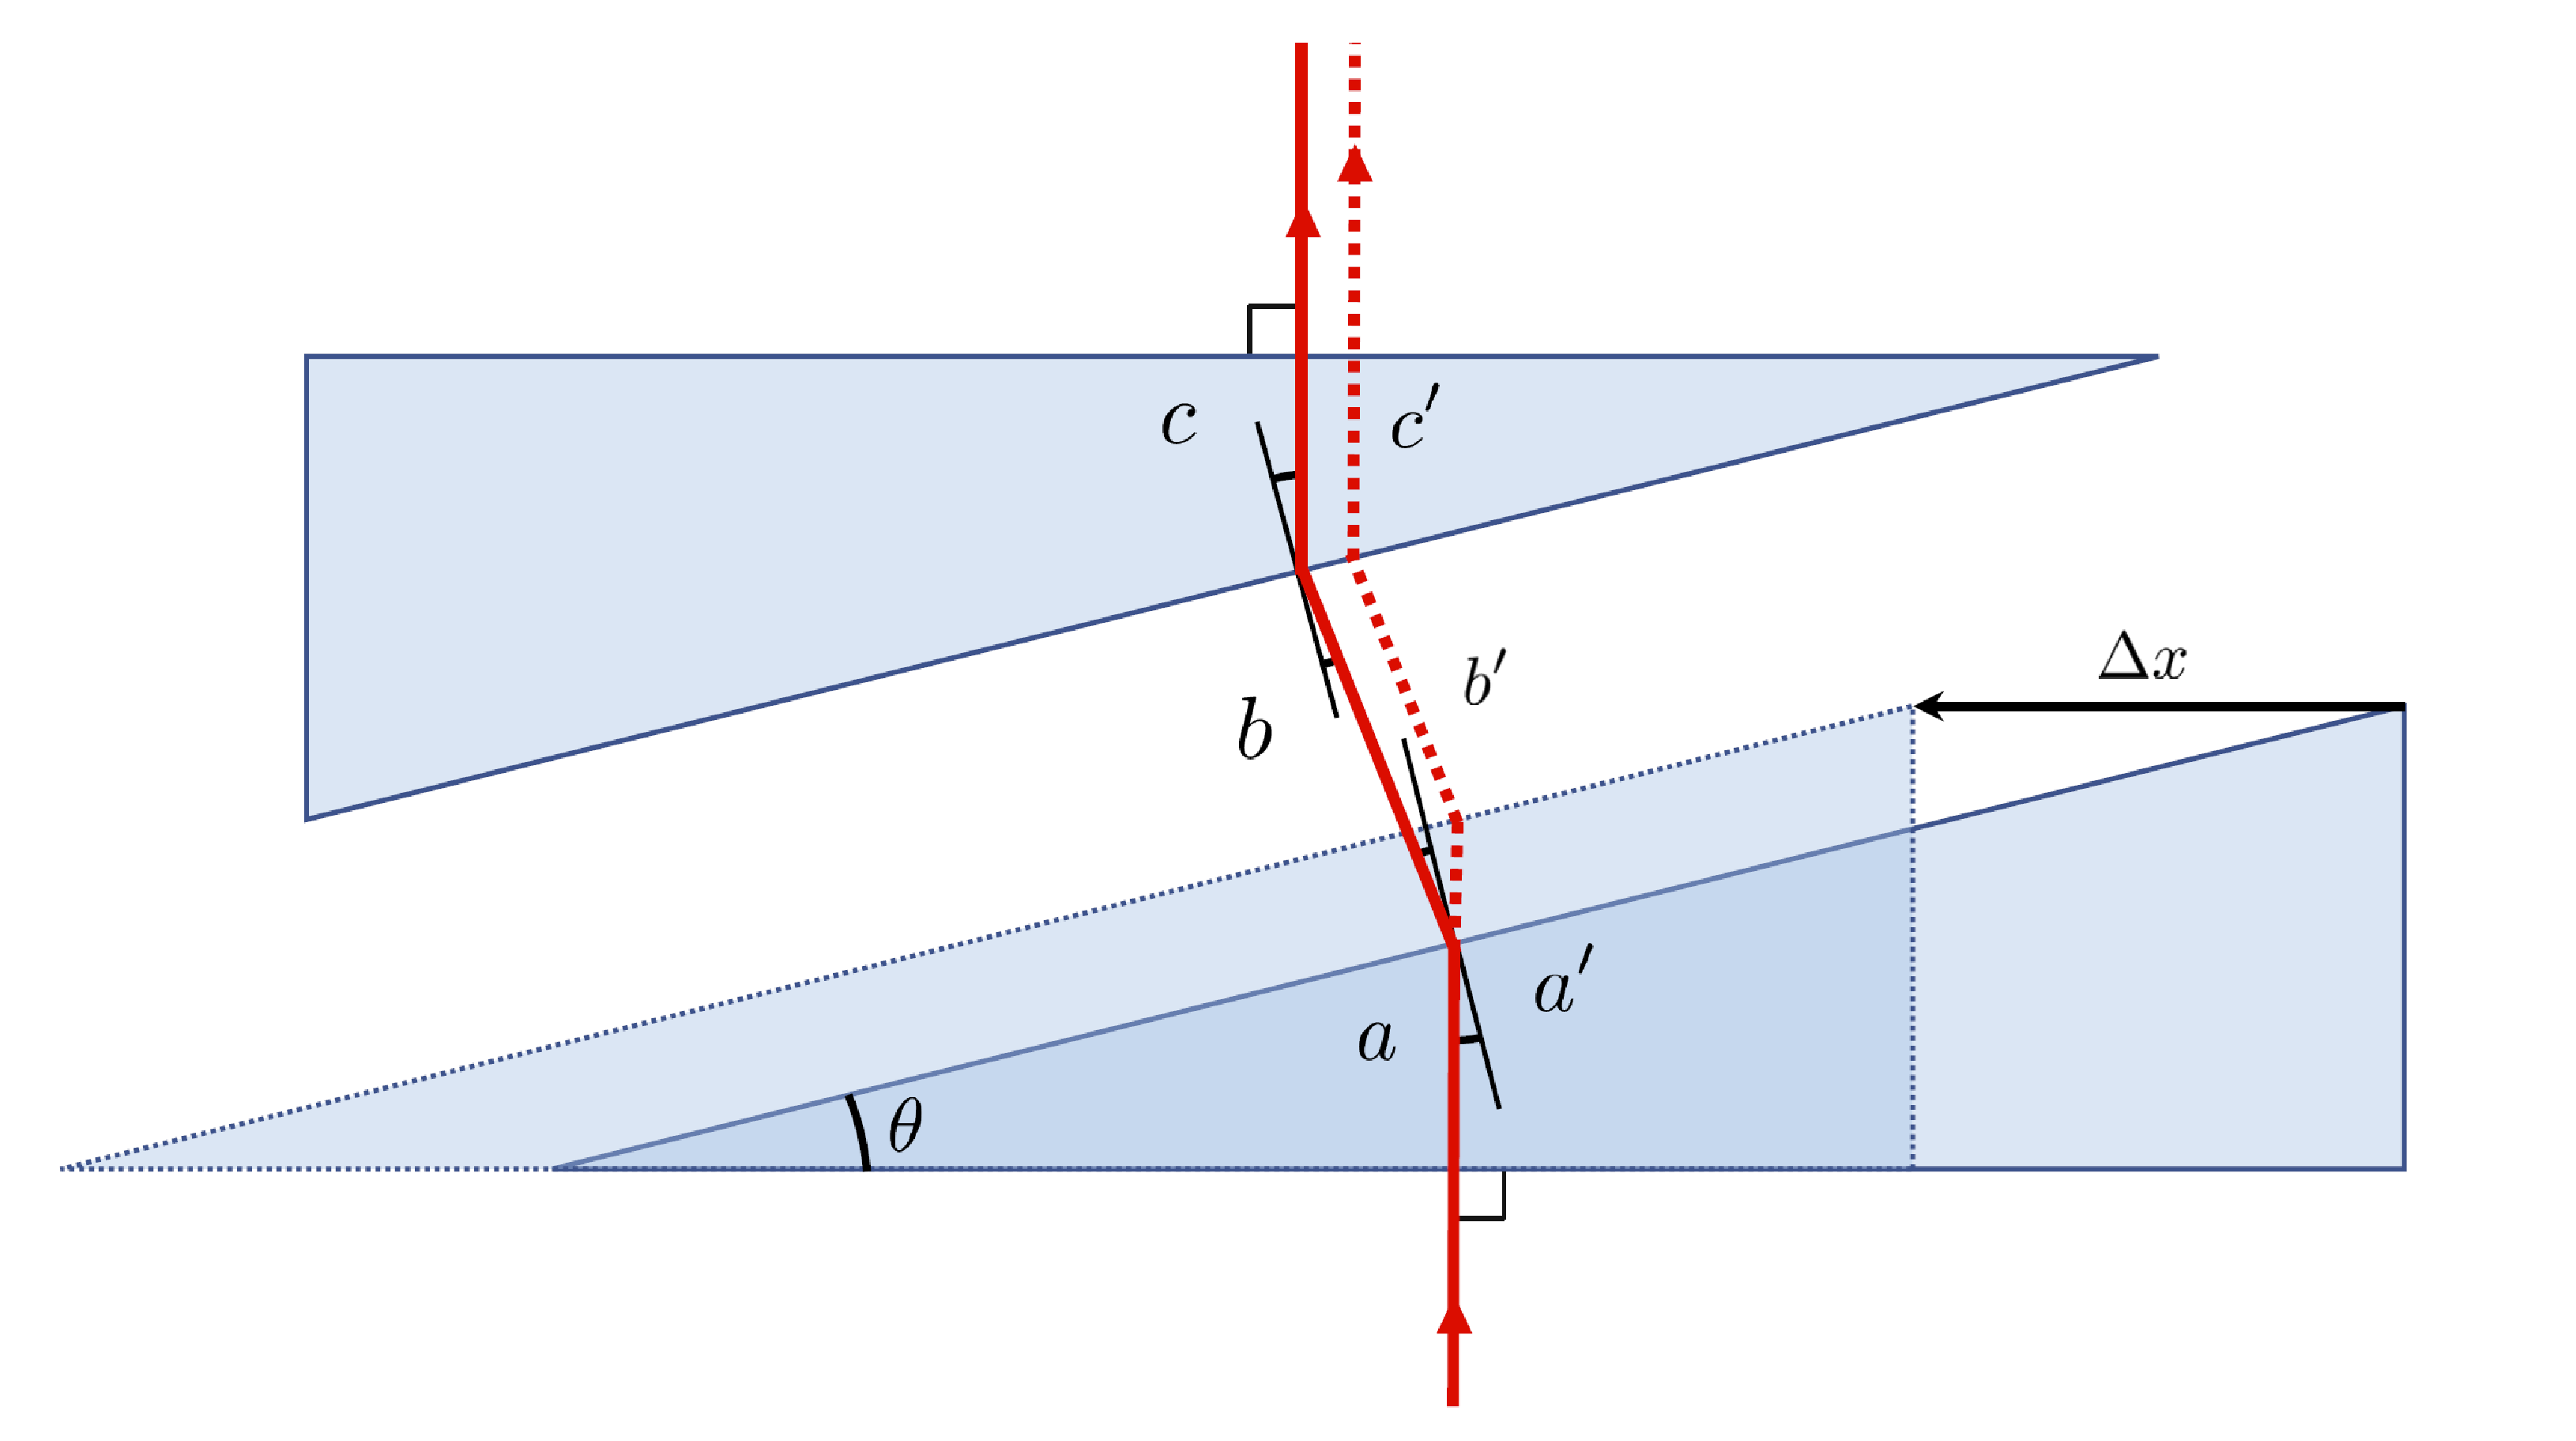
\includegraphics[width=0.8\textwidth]{figures/Beamline/wedge_calibration.pdf}
	\caption{Schematic of the FS wedges used to control the time delay between the IR and XUV pulses in the dressing and generation arms interferometer, respectively. The wedges are aligned such that the input beam is normal to the first wedge face, and the beam exits the wedges normal to the last face of the second wedge.  Only one of the wedges is motorized and is shown before and after a displacement by an amount $\Delta x$.}
	\label{fig:wedges}
\end{figure}


\begin{align}
	a'&=a+\Delta x \tan\theta\\
	b'&=b-\Delta x \bigg(\frac{\sin\theta}{\cos\psi}\bigg)\\
	c'&=c-\Delta x \tan\theta\sin\theta\frac{\cos(\frac{\pi}{4})+\psi}{\sin(\frac{\pi}{4}+\theta+\psi)}
\end{align}

where
\begin{equation}
	\psi = \arcsin(n\sin\theta)
\end{equation}

\begin{equation}
\label{eqn:time_delay}
	\Delta\tau = \frac{\Delta x}{c}\Bigg[(n-1)\tan\theta - \frac{\sin\theta}{\cos\psi}-(n-1)\tan\theta\sin\theta\bigg(\frac{\cos(\frac{\pi}{4})+\psi}{\sin(\frac{\pi}{4}+\theta+\psi)}\bigg)\Bigg]
\end{equation}

\section{Photon Spectrometer}
\label{sec:photon_spec}
\subsection{Spectrometer Calibration}
\label{subsec:spec_calibration}